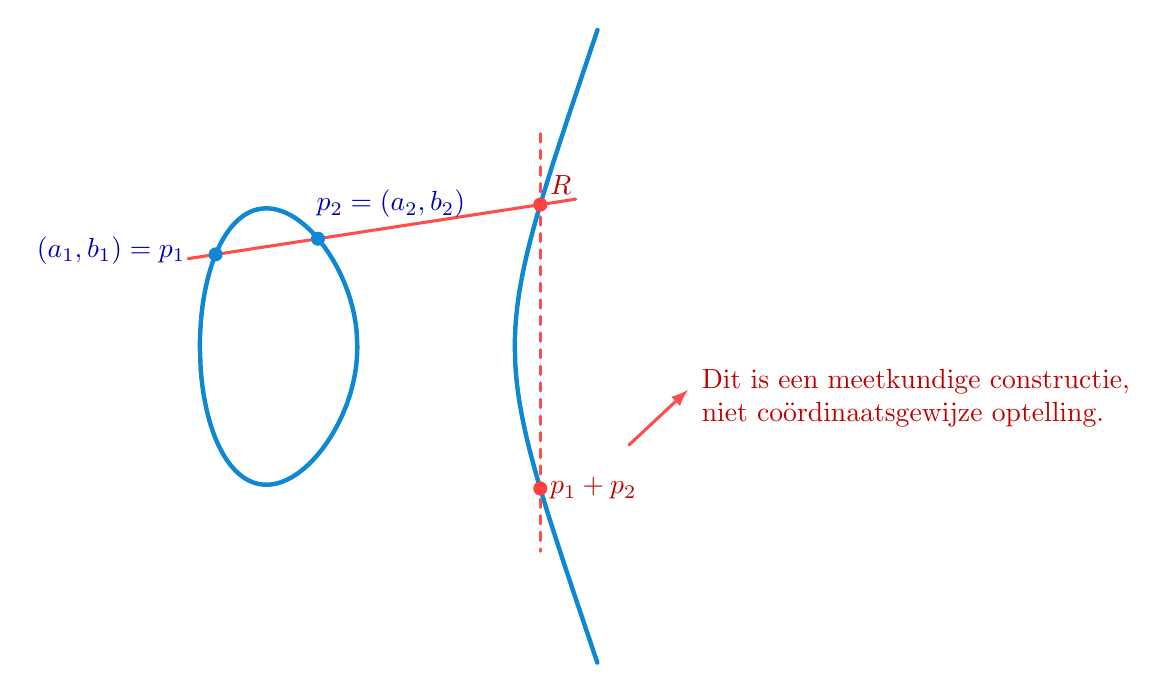
\begin{tikzpicture}[>=latex, line cap=round, line join=round]

% --- Global TikZ Styles ---
\tikzset{
    elliptic/.style={
        draw=cyan!70!blue,
        line width=1.6pt
    },
    construction/.style={
        draw=red!70,
        line width=1.1pt
    },
    constructiondashed/.style={
        draw=red!70,
        dashed,
        line width=1.1pt
    },
    bluepoint/.style={
        circle,
        fill=cyan!70!blue,
        inner sep=1.8pt
    },
    redpoint/.style={
        circle,
        fill=red!75,
        inner sep=1.8pt
    }
}

% =========================================================================
% --- Basisgeval groepswet op elliptische kromme ---
% =========================================================================

% We gebruiken dezelfde kromme als je rechterfiguur:
% y^2 = x^3 - 4x, verschoven met -1.2 in de x-richting.

\pgfmathsetmacro{\curveShift}{-1.2}

% --- Kies twee punten op de gesloten component ---
\pgfmathsetmacro{\xPone}{-1.80}
\pgfmathsetmacro{\yPone}{sqrt(abs(\xPone*\xPone*\xPone - 4*\xPone))}

\pgfmathsetmacro{\xPtwo}{-0.50}
\pgfmathsetmacro{\yPtwo}{sqrt(abs(\xPtwo*\xPtwo*\xPtwo - 4*\xPtwo))}

% --- Lijn door p_1 en p_2 ---
\pgfmathsetmacro{\msec}{(\yPtwo-\yPone)/(\xPtwo-\xPone)}
\pgfmathsetmacro{\csec}{\yPone-\msec*\xPone}

% --- Derde snijpunt R met de kromme ---
% Voor y^2 = x^3 - 4x geldt: x_R = m^2 - x_1 - x_2
\pgfmathsetmacro{\xRraw}{\msec*\msec-\xPone-\xPtwo}
\pgfmathsetmacro{\yR}{\msec*\xRraw+\csec}

% --- Verschoven x-coördinaten voor tekenen ---
\pgfmathsetmacro{\XPone}{\xPone+\curveShift}
\pgfmathsetmacro{\XPtwo}{\xPtwo+\curveShift}
\pgfmathsetmacro{\XR}{\xRraw+\curveShift}

% --- Eindpunten van de rode secantlijn ---
\pgfmathsetmacro{\lineStartX}{\XPone-0.35}
\pgfmathsetmacro{\lineStartY}{\yPone-\msec*0.35}
\pgfmathsetmacro{\lineEndX}{\XR+0.45}
\pgfmathsetmacro{\lineEndY}{\yR+\msec*0.45}

% --- Gesloten ovaalcomponent ---
\draw[elliptic]
    plot[domain=0:-2, samples=200]
        (\x + \curveShift, {sqrt(abs(\x*\x*\x - 4*\x))})
    --
    plot[domain=-2:0, samples=200]
        (\x + \curveShift, {-sqrt(abs(\x*\x*\x - 4*\x))})
    -- cycle;

% --- Rechter oneindige component ---
\draw[elliptic]
    plot[domain=3.05:2, samples=200]
        (\x + \curveShift, {sqrt(abs(\x*\x*\x - 4*\x))})
    --
    plot[domain=2:3.05, samples=200]
        (\x + \curveShift, {-sqrt(abs(\x*\x*\x - 4*\x))});

% --- Rode secantlijn door p_1 en p_2 ---
\draw[construction]
    (\lineStartX,\lineStartY) -- (\lineEndX,\lineEndY);

% --- Verticale spiegelingslijn door R ---
\draw[constructiondashed]
    (\XR,{\yR+0.9}) -- (\XR,{-\yR-0.8});

% --- Punten ---
\node[bluepoint] at (\XPone,\yPone) {};
\node[bluepoint] at (\XPtwo,\yPtwo) {};
\node[redpoint] at (\XR,\yR) {};
\node[redpoint] at (\XR,{-\yR}) {};

% --- Labels ---
\node[blue!70!black, left, xshift=-6pt] at ({\XPone-0.05},{\yPone+0.05})
    {$(a_1,b_1)=p_1$};

\node[blue!70!black, above right, yshift=4pt, xshift=-4pt] at (\XPtwo,\yPtwo)
    {$p_2=(a_2,b_2)$};

\node[red!75!black, above right] at (\XR,\yR)
    {$R$};

\node[red!75!black, right] at (\XR,{-\yR})
    {$p_1+p_2$};

% --- Opmerking rechts ---
\draw[construction, ->]
    (2.25,-1.25) -- (3.0,-0.55);
    %(3.0,-0.55) -- (2.25,-1.25);

\node[red!75!black, align=left, right] at (3.05,-0.65)
    {Dit is een meetkundige constructie,\\
     niet coördinaatsgewijze optelling.};

\end{tikzpicture}